% \usepackage{xcolor}
% \usepackage{afterpage}
\usepackage{pifont,mdframed}
% \usepackage{wrapfig}
% \usepackage[bottom]{footmisc}

\makeatletter
\gdef\this@inputfilename{input.txt}
\gdef\this@outputfilename{output.txt}
\makeatother

\newcommand{\inputfile}{\texttt{input.txt}}
\newcommand{\outputfile}{\texttt{output.txt}}

\newenvironment{warning}
  {\par\begin{mdframed}[linewidth=2pt,linecolor=gray]%
    \begin{list}{}{\leftmargin=1cm
                   \labelwidth=\leftmargin}\item[\Large\ding{43}]}
  {\end{list}\end{mdframed}\par}

	\begin{wrapfigure}{r}{7cm}
	\centering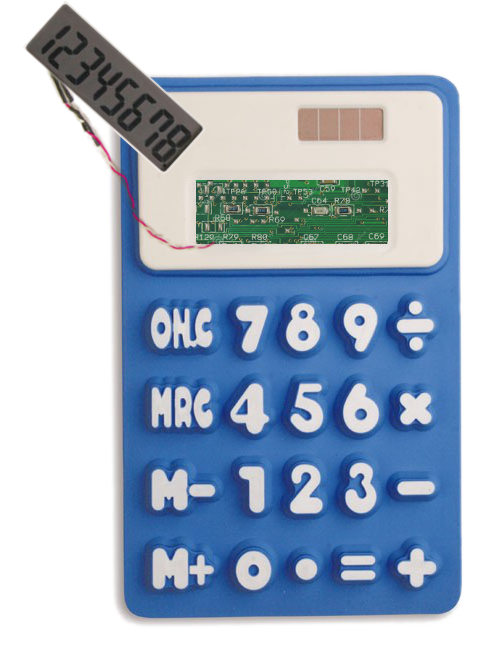
\includegraphics[width=7cm]{calcolatrice.png}
%	\caption{\small{Rappresentazione artistica della calcolatrice di Giorgio.}}
	\end{wrapfigure}

	La calcolatrice che Giorgio conserva gelosamente da quando faceva le elementari si è rotta, e ora il suo schermo \emph{LCD} vecchio stile penzola appeso ai tasti dal solo filo di alimentazione. Nonostante questo, funziona ancora perfettamente come un tempo e quindi Giorgio non ha intenzione di smettere di utilizzarla.

	Con la sua affezionata calcolatrice, Giorgio ha appena fatto dei lunghi e complessi calcoli i cui risultati potrebbero portare alla soluzione di numerose congetture in innumerevoli campi della matematica, e ne ha trascritto i risultati su un foglio. Tuttavia solo dopo si è accorto che, per via del danno descritto sopra, non è in grado di capire l'orientamento giusto dello schermo e quindi in alcuni casi potrebbe aver trascritto il risultato sbagliato (e cioè come si leggerebbe ruotando lo schermo della calcolatrice di $180^\circ$).

	Da un'approssimazione a stima che si è fatto, gli sembra che i risultati dovrebbero essere numeri abbastanza piccoli. Pertanto, dato un numero $N$, vuole scrivere un programma che calcoli il corrispondente numero $M$ ruotato di $180^\circ$, e se questo è effettivamente un numero sensato scelga il minore tra i due.

\Implementation
Dovrai sottoporre esattamente un file con estensione \texttt{.c}, \texttt{.cpp} o \texttt{.pas}.

\begin{warning}
Tra gli allegati a questo task troverai un template (\texttt{calcolatrice.c}, \texttt{calcolatrice.cpp}, \texttt{calcolatrice.pas}) con un esempio di implementazione da completare.
\end{warning}

Se sceglierai di utilizzare il template, dovrai implementare la seguente funzione:
\begin{center}\begin{tabularx}{\textwidth}{|c|X|}
\hline
C/C++  & \verb|int rimedia(int N);|\\
\hline
Pascal & \verb|function rimedia(N: longint): longint;|\\
\hline
\end{tabularx}\end{center}
In cui:
\begin{itemize}[nolistsep]
  \item L'intero $N$ rappresenta il numero segnato sul foglio da Giorgio.
  \item La funzione dovrà restituire il minimo tra $N$ e il corrispondente $M$ ruotato di $180^\circ$ (se sensato), che verrà stampato sul file di output.
\end{itemize}

\InputFile
Il file \inputfile{} è composto da un'unica riga contenente l'unico intero $N$.

\OutputFile
Il file \outputfile{} è composto da un'unica riga contenente un unico intero, la risposta a questo problema.

% Assunzioni
\Constraints
\begin{itemize}[nolistsep, itemsep=2mm]
	\item $0 \le N \le 1\,000\,000\,000$.
\end{itemize}

\Scoring
Il tuo programma verrà testato su diversi test case raggruppati in subtask.
Per ottenere il punteggio relativo ad un subtask, è necessario risolvere
correttamente tutti i test relativi ad esso.

\begin{itemize}[nolistsep,itemsep=2mm]
  \item \textbf{\makebox[2cm][l]{Subtask 1} [10 punti]}: Casi d'esempio.
  \item \textbf{\makebox[2cm][l]{Subtask 2} [20 punti]}: $N \leq 10$.
  \item \textbf{\makebox[2cm][l]{Subtask 3} [30 punti]}: $N \leq 100$.
  \item \textbf{\makebox[2cm][l]{Subtask 4} [40 punti]}: Nessuna limitazione specifica.
\end{itemize}

% Esempi
\Examples
\begin{example}
\exmp{
14
}{%
14
}%
\end{example}
\begin{example}
\exmp{
12650
}{%
12650
}%
\end{example}
\begin{example}
\exmp{
806129
}{%
621908
}%
\end{example}


\Explanation
Nel \textbf{primo caso di esempio}, il numero \texttt{14} ruotato non genera un numero sensato, per via della presenza della cifra \texttt{4}.\\[2mm]
Nel \textbf{secondo caso di esempio}, il numero \texttt{12650} ruotato genera il numero \texttt{05921} che non è da considerarsi sensato, per via della presenza della cifra \texttt{0} come prima cifra.\\[2mm]
Nel \textbf{terzo caso di esempio}, il numero \texttt{806129} ruotato genera il numero \texttt{621908} che è sensato e minore del precedente.
